



\tikzset{every picture/.style={line width=0.75pt}} %set default line width to 0.75pt        

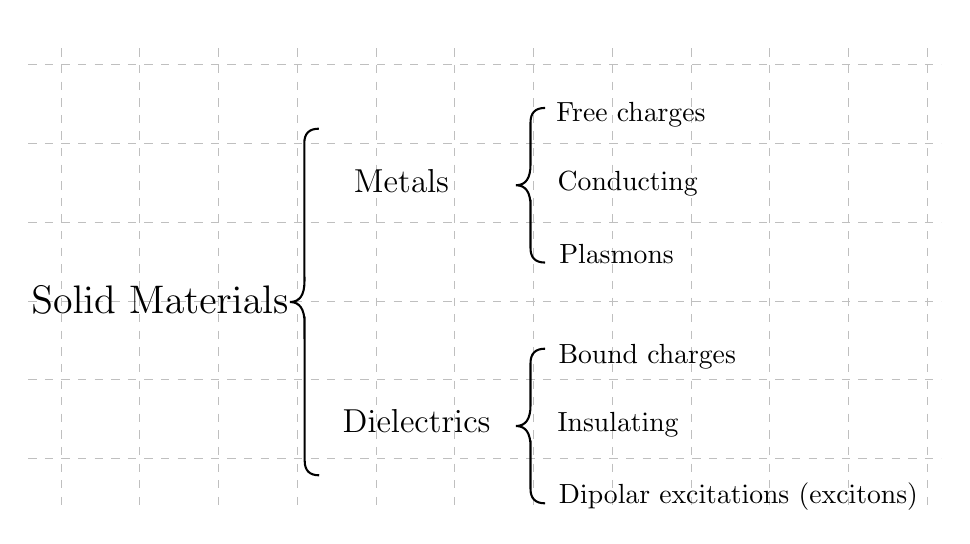
\begin{tikzpicture}[x=0.75pt,y=0.75pt,yscale=-1,xscale=1,remember picture]
%uncomment if require: \path (0,300); %set diagram left start at 0, and has height of 300
\draw[lightgray,thin,dashed] (60,30)  grid  (500,250);
\useasboundingbox (60,20) rectangle (500,255);

\begin{scope}[yshift={9.5}]
    %\fill[fill=blue!10] (60,30) rectangle (500,250);
%Shape: Brace [id:dp45369403742662895] 
\draw<2->   (200,56) .. controls (195.33,56.01) and (193,58.34) .. (193.01,63.01) -- (193.09,129.51) .. controls (193.1,136.18) and (190.77,139.51) .. (186.1,139.52) .. controls (190.77,139.51) and (193.1,142.84) .. (193.11,149.51)(193.11,146.51) -- (193.2,216.01) .. controls (193.2,220.68) and (195.53,223.01) .. (200.2,223) ;
%Shape: Brace [id:dp9306672772670488] 
\draw<5->   (309,46) .. controls (304.33,46) and (302,48.33) .. (302,53) -- (302,73.25) .. controls (302,79.92) and (299.67,83.25) .. (295,83.25) .. controls (299.67,83.25) and (302,86.58) .. (302,93.25)(302,90.25) -- (302,113.5) .. controls (302,118.17) and (304.33,120.5) .. (309,120.5) ;
%Shape: Brace [id:dp8400849826669508] 
\draw<9->   (309,162) .. controls (304.33,162) and (302,164.33) .. (302,169) -- (302,189.25) .. controls (302,195.92) and (299.67,199.25) .. (295,199.25) .. controls (299.67,199.25) and (302,202.58) .. (302,209.25)(302,206.25) -- (302,229.5) .. controls (302,234.17) and (304.33,236.5) .. (309,236.5) ;

% \draw (200.,87.) -- (340,87.);
% \draw (200.,203.0) -- (340,203.0);

% Text Node
\draw<1-> (60,130) node [anchor=north west][inner sep=0.75pt]  [font=\Large] [align=left] {Solid Materials};
% Text Node
\draw<3-> (215.4,74.) node [anchor=north west][inner sep=0.75pt]  [font=\large] [align=left] {Metals};
% Text Node
\draw<4-> (210,190.0) node [anchor=north west][inner sep=0.75pt]  [font=\large] [align=left] {Dielectrics};
% Text Node
\draw<6-> (313,42.0) node [anchor=north west][inner sep=0.75pt]   [align=left] {Free charges};
% Text Node
\draw<7-> (313.6,75.) node [anchor=north west][inner sep=0.75pt]   [align=left] {Conducting};
% Text Node
\draw<8-> (314.4,110) node [anchor=north west][inner sep=0.75pt]   [align=left] {Plasmons};
% Text Node
\draw<10-> (314,158.6) node [anchor=north west][inner sep=0.75pt]   [align=left] {Bound charges};
% Text Node
\draw<11-> (313.6,191.0) node [anchor=north west][inner sep=0.75pt]   [align=left] {Insulating};
% Text Node
\draw<12-> (314.2,225.0) node [anchor=north west][inner sep=0.75pt]   [align=left] {Dipolar excitations (excitons)};
\end{scope}

\end{tikzpicture}